\section{Experiments} \label{sec:experiments}
In this section, we present our test-time experimental setup used to evaluate the DP framework under varying conditions
and introduce some points of discussion we found relevant and decided to explore further.

In Section~\ref{sec:pretrained_model}, we begin by describing the pre-trained LeRobot model we use for the Push-T environment.
We then detail how we managed to train our own models from scratch in Section~\ref{sec:training_model}.
In Section~\ref{sec:tradeoff_denoising_steps}, we briefly discuss the trade-off between the number of denoising
steps and the model's performance.
Next, in Section~\ref{sec:action_multimodality}, we investigate the agent's behavior in multimodal scenarios, where multiple valid action trajectories are possible (e.g. bypass the T by the left or right).
Finally, in Section~\ref{sec:visual_perturbations}, we detail the evaluation protocols and experimental setup used to introduce and measure the impact of visual perturbations on the policy's performance.

\subsection{LeRobot's Pre-Trained Action Diffusion Model}\label{sec:pretrained_model}

While the authors of the original DP article have made their code available, a recent and more
accessible implementation has been provided by Hugging Face through their LeRobot
framework~\cite{cadene2024lerobot}.

Our first experiments were based on a pre-trained diffusion policy model provided by the LeRobot team
and applied to the Push-T environment
\footnote{Available at \url{https://github.com/huggingface/gym-pusht}}.
The goal of this task is to push a T-shaped block to a fixed target location in a 2D space. There are two
ways of assessing the agent's performance: the success rate and the average maximum overlap between the
object and the target. To be considered successful, the object must overlap the target by at least 95\%.

While the original DP authors proposed two implementations, a Transformer-based and a CNN-based architecture,
only the latter is available in the LeRobot library.
Visual observations are processed using a ResNet-18 encoder trained from scratch (i.e., without ImageNet
pretraining), transforming raw RGB inputs into compact feature vectors.
These observation features condition the diffusion process that sequentially predicts actions, which are
end-effector positions.
This diffusion-based policy has been trained from 206 human demonstrations
\footnote{Collected via \url{https://github.com/real-stanford/diffusion_policy}}, for 7 hours on
an Nvidia RTX 3090.
More precisely, it consists of 200k steps of training with a batch size of 32, using various data
augmentation techniques (image brightness, contrast, saturation, hue and sharpness).

Figure~\ref{fig:coverage_illustration} illustrates three possible outcomes with different object-to-target
coverage levels.
\begin{figure}[!htb]
    \centering
    \begin{subfigure}[b]{0.4\linewidth}
        \centering
        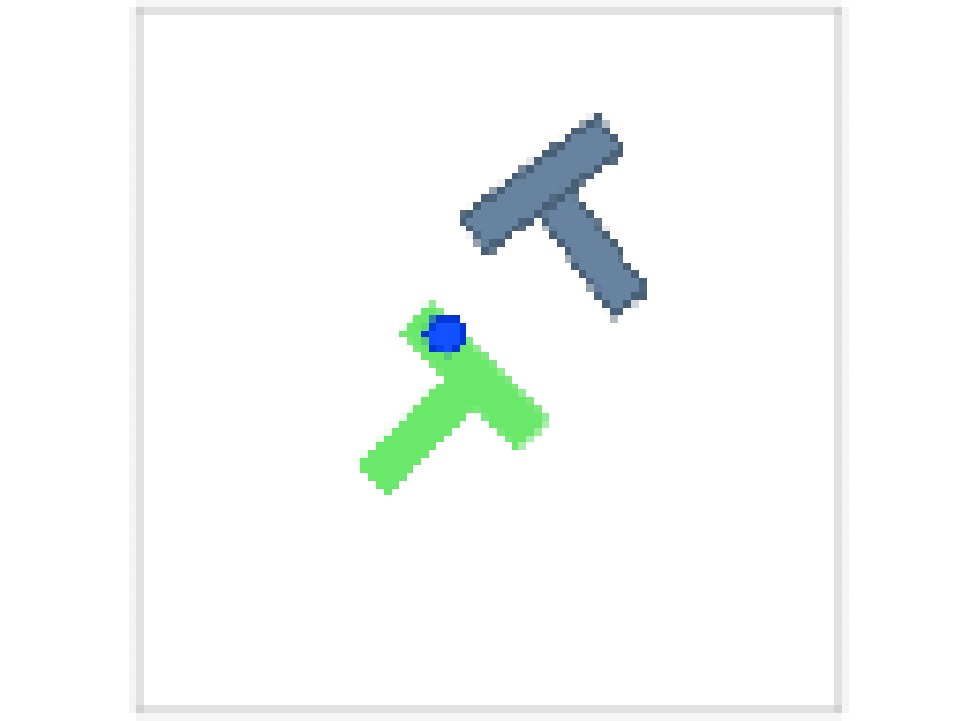
\includegraphics[width=\linewidth]{figures/illustration_0.pdf}
        \caption{No coverage ($\approx 0.0\%$)}
    \end{subfigure}

    \begin{subfigure}[b]{0.4\linewidth}
        \centering
        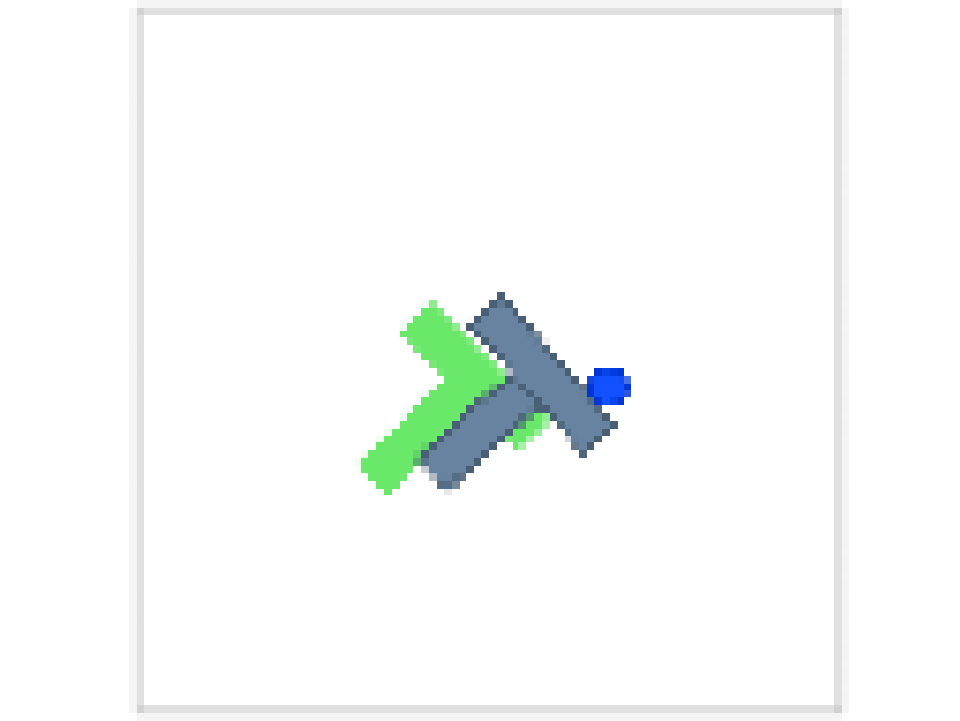
\includegraphics[width=\linewidth]{figures/illustration_50.pdf}
        \caption{Low coverage ($\approx 16\%$)}
    \end{subfigure}
    \begin{subfigure}[b]{0.4\linewidth}
        \centering
        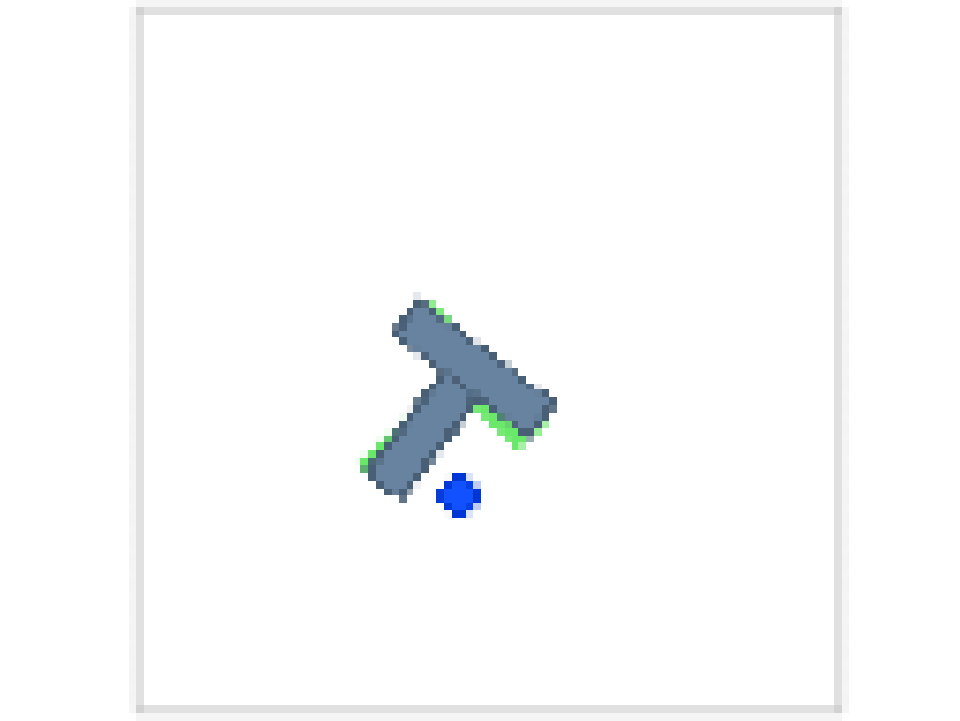
\includegraphics[width=\linewidth]{figures/illustration_150.pdf}
        \caption{High coverage ($\approx 89\%$)}
    \end{subfigure}
    \caption{Illustrations of different object-to-target coverage levels obtained by the LeRobot pre-trained diffusion policy on the Push-T task.}
    \label{fig:coverage_illustration}
\end{figure}
The evaluation results\footnote{Available at \url{https://huggingface.co/lerobot/diffusion_pusht}} of
the LeRobot's implementation compared to a CNN-based architecture similar to the original DP article are
summarized in Table~\ref{tab:evaluation_results}.
\begin{table}[!htb]
    \centering
    \begin{tabular}{lcc}
    \hline
    Metric & HF & DP \\
    \hline
    Average max. overlap (\%) & 95.9 & 95.7 \\
    Success rate (\%) & 63.8 & 64.2 \\
    % Beta distribution lower/mean/upper (\%) & 61.6 / 63.7 / 65.9 & 62.0 / 64.1 / 66.3 \\
    \hline
    \end{tabular}
    \caption{Evaluation results of the pre-trained diffusion policy model (`DP') compared to the LeRobot implementation (`HF'). Metrics are computed over 500 evaluation episodes.}
    \label{tab:evaluation_results}
\end{table}
We observe a gap of nearly 20\% in success rate compared to the results presented in the paper.
We are not able to explain this difference, as the original training used less training samples and
the exact same architecture.

\subsection{Training our own models}\label{sec:training_model}

For a more in-depth understanding of the DP framework, we wanted to train a diffusion policy model from scratch.
However, due to the high computational cost of training such models, we were unable to complete this task
with our limited resources. We decided to reduce the number of training steps and benefit from Kaggle's
free GPU resources (30h hours per week per user on a Nvidia Tesla P100 GPU) to train a model
on the Push-T environment for few hours. We observed that at least 5k
steps are required to obtain a policy not too fuzzy. In this case, the success rate is not an appropriate
metric anymore, as it is hard for the policy to reach a 95\% overlap. We then decided to use the average
maximum overlap as the main evaluation metric.

\subsection{Number of denoising steps: a first trade-off}\label{sec:tradeoff_denoising_steps}

When dealing with diffusion models, the number of denoising steps is a crucial hyperparameter that can
impact the model's performance. Ideally, one would set this parameter as high as possible to ensure
the best possible denoising. However, this comes at the cost of increased computational complexity, which
can be prohibitive at test time for real-time applications. As mentioned previously, the DDIM framework
allows us to use a much lower number of denoising steps at inference than during training, but we
may be able to do better. We conducted a simple qualitative experiment by increasing the number of
denoising steps at inference time and analysed the influence on a batch of generated sequences. With a
single denoising step, the generated sequences are still very noisy (Figure \ref{fig:single_denoising_step}).
By increasing the number of denoising steps, the sequences become more coherent and gather around a
common trajectory. In order to quantify this observation, we computed the standard deviation of the
batch of predicted actions at each time step for different numbers of denoising steps (Figure
\ref{fig:heatmap_denoising_steps}). From 2 steps, the standard deviation is already significantly reduced,
but we chose to use at least 10 steps during our experiments for a less noisy policy. Whatsmore, note
that it is quite rare to have an important spread of the predicted actions at certain time steps, which
suggests that the policy is quite confident in its predictions. We would expect a large standard deviation
when multiple actions are possible to reach the goal (multimodality) or when we are out of the
training distribution.
\begin{figure*}[!htb]
    \begin{subfigure}[b]{0.65\linewidth}
        \centering
        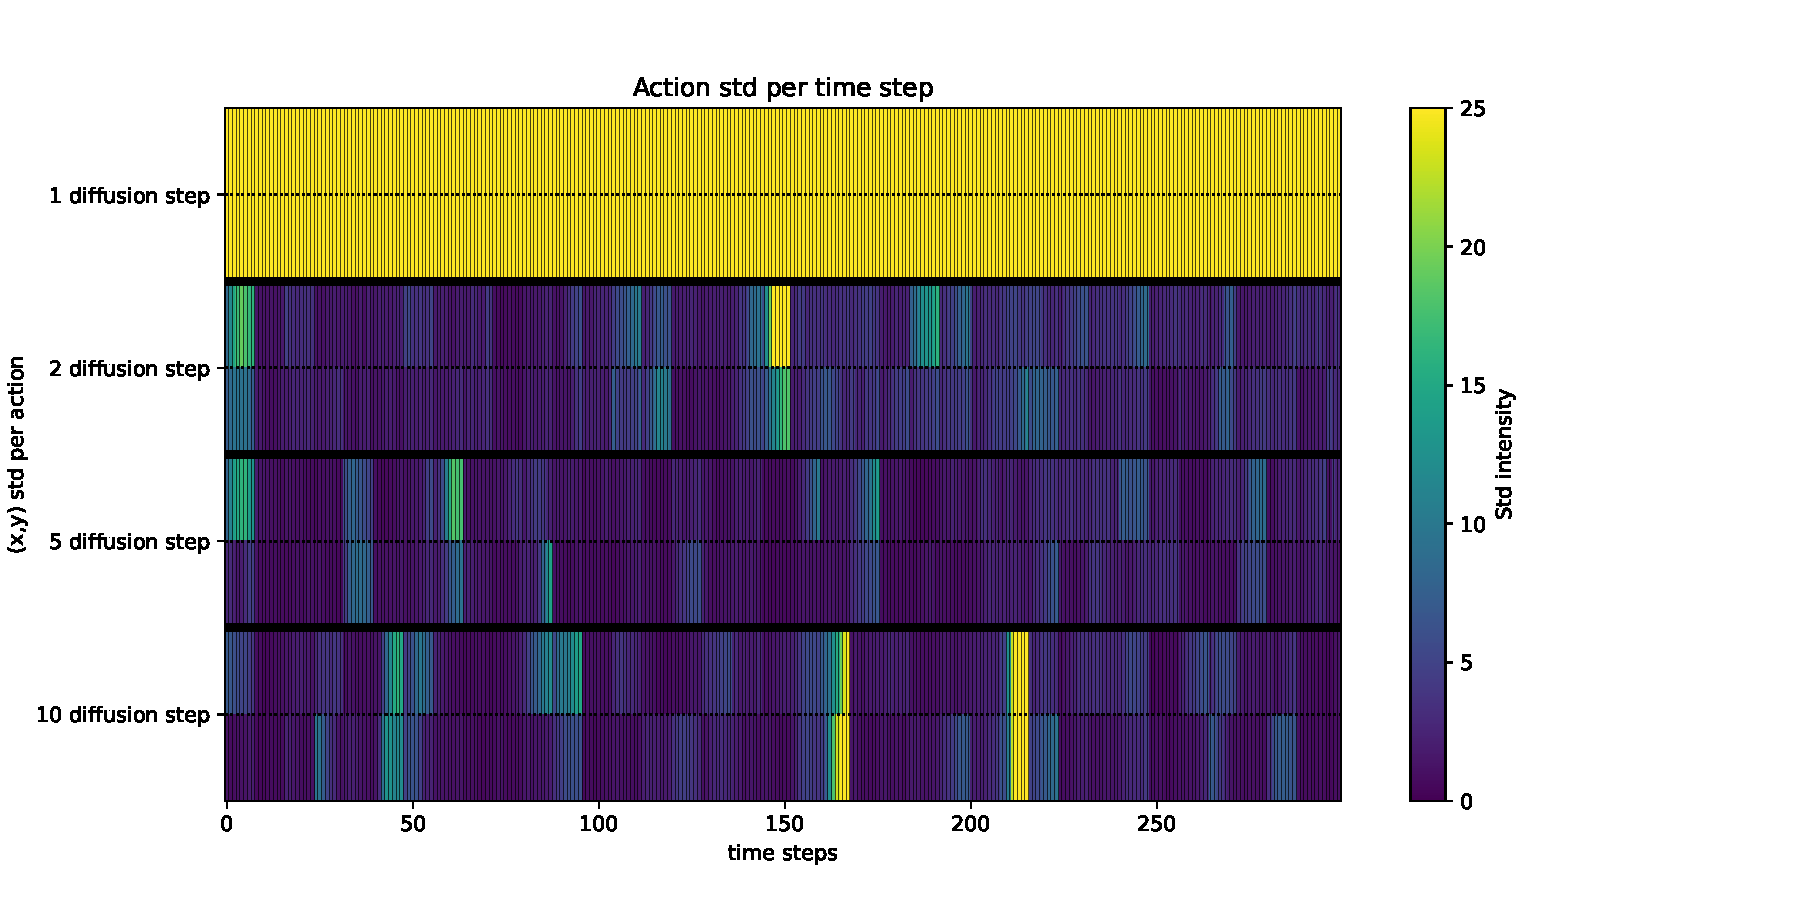
\includegraphics[width=\linewidth]{figures/plot_heatmap.pdf}
        \caption{Standard deviation of the predicted actions (thresholded at 25 pixels).}
        \label{fig:heatmap_denoising_steps}
    \end{subfigure}
    \begin{subfigure}[b]{0.34\linewidth}
        \centering
        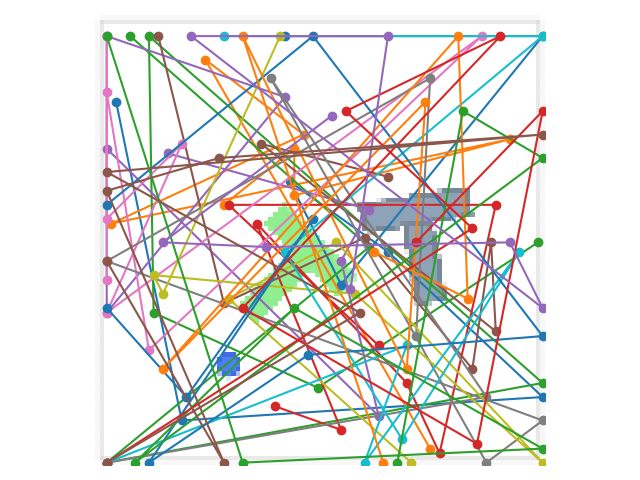
\includegraphics[width=\linewidth]{figures/random_actions.png}
        \caption{Generated action sequences with a single denoising step in a $96 \times 96$ action space.}
        \label{fig:single_denoising_step}
    \end{subfigure}
    \caption{Influence of the number of denoising steps on the generated action sequences.}
    \label{fig:number_denoising_steps}
\end{figure*}

\subsection{Focus on action multimodality}\label{sec:action_multimodality}
% \TODO{
%     Tom, On met un premier descriptif ici avec les trois images du poster, et on trouve quelque chose de plus qualitatif pour la section suivante ?
%     Ou on en parle ici seulement, et on change le titre de la section ?
%     On peut aussi faire une section dédiée pour parler de ça: Abstract, Introduction, Method, LeRobot framework, Study of action multimodality, Visual Perturbations + Results, overcoming the patch problem, conclusion ?
%     C'est un rapport et pas un article après tout, donc on peut se le permettre...}

Action multimodality is a common issue in visuomotor policy learning. It refers to the presence of multiple
valid action trajectories that can lead to the same goal. In a scenario involving multimodality, we want the
agent to execute one of the possible actions, but ideally, we would like it to know the different options
and choose the best one.

We replicated such a scenario in the Push-T environment by aligning the agent with the object and the target
(Figure \ref{fig:multimodality_experiment}). We predicted multiple action sequences from different initial
noisy sequences and progressively shifted the agent's position to the right, parallel to the T bar.
\begin{figure}[!htb]
    \centering
    \begin{subfigure}[b]{0.4\linewidth}
        \centering
        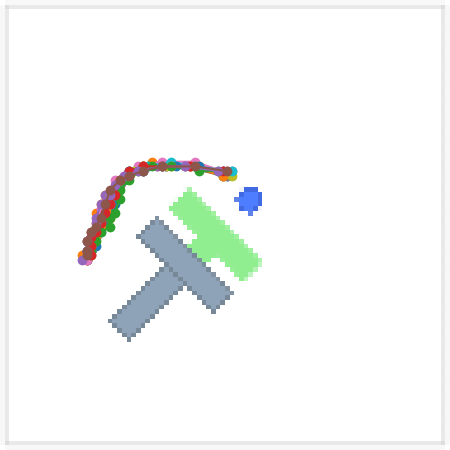
\includegraphics[width=\linewidth]{figures/multimodality_centered.png}
        \caption{Centered}
    \end{subfigure}

    \begin{subfigure}[b]{0.4\linewidth}
        \centering
        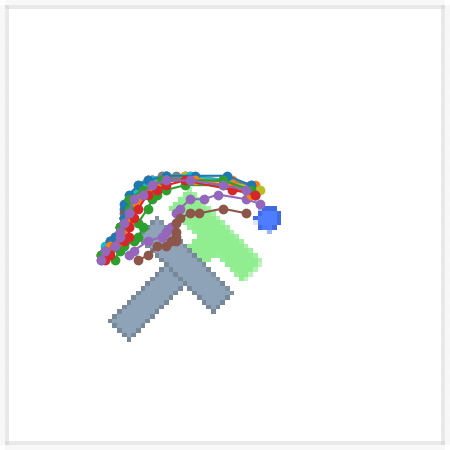
\includegraphics[width=\linewidth]{figures/multimodality_shifted.png}
        \caption{Shifted to the right}
    \end{subfigure}
    \begin{subfigure}[b]{0.4\linewidth}
        \centering
        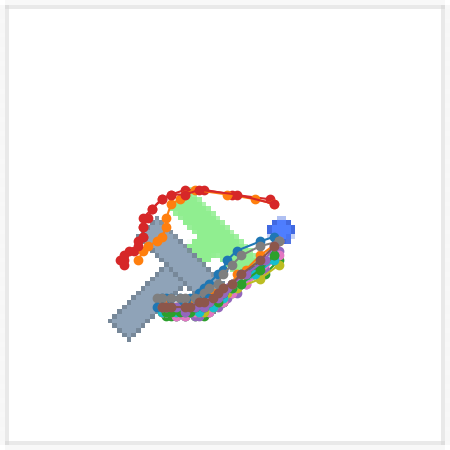
\includegraphics[width=\linewidth]{figures/multimodality_shifted+.png}
        \caption{Shifted further to the right}
    \end{subfigure}
    \caption{Generated actions while shifting the agent's position parallel to the T bar.}
    \label{fig:multimodality_experiment}
\end{figure}
We observe that DP is able to deal with multimodality-related decision ambiguities but is suboptimal: the agent
favors the left side to bypass the T, while the right side is also a valid option. We need to shift the agent
sufficiently to the right to make it choose the right side.
As the human providing the demonstrations is not an expert, suboptimality is an inherent issue.
The demonstrations could be biased and/or not provide enough data to cover all possible scenarios.
Another explanation, that we believe is less likely, is that the model is not expressive enough to capture
the complexity of the underlying multimodal distribution it tries to sample from.


\subsection{Visual perturbations on the input images}\label{sec:visual_perturbations}

To evaluate the visual robustness of the pre-trained diffusion policy, we apply controlled perturbations to the input image observations at test time.
These perturbations simulate realistic challenges such as camera noise, or environmental distractions (e.g. waving hand in front of the camera).
Beyond robustness to visual perturbations, which largely depends on the data and augmentations used
during training, we wanted to more broadly observe the behavior of DP when it encounters situations
outside the training distribution.
Detecting such situations and adapting the method is a key challenge for real-world applications.
Illustrated in Figure~\ref{fig:visual_perturbations_examples}, the following scenarios are considered:

\paragraph{(1) No Perturbation:}
Figure~\ref{fig:visual_perturbations_examples_clean} shows this baseline condition, where the input image stream remains unaltered.
This scenario provides a reference point for the model's expected performance under ideal visual conditions and helps us quantify any degradation resulting from additional disturbances.

\paragraph{(2) Gaussian Noise:}
To simulate sensor-level noise and low-quality vision input, we corrupt the input images by adding Gaussian noise with zero mean and a standard deviation of $0.1$.
Assuming the input pixels are normalized to the [0, 1] range, this corresponds to a 10\% intensity-level noise degradation.
Figure~\ref{fig:visual_perturbations_examples_noise} illustrates this condition.
% Such a level of noise allows us to measure the policy's ability to maintain performance despite reduced image clarity, contrast, and signal-to-noise ratio.

\paragraph{(3) Black Patch Occlusion:}
Inspired by the original DP article \cite{chi2023diffusion}, we insert a fixed-size black patch, $10\times10$ pixels, over random regions of the input image as shown by Figure~\ref{fig:visual_perturbations_examples_patch}.
This occlusion simulates dynamic occlusions that might occur, for example, when a human hand passes in front of the camera.
Such partial visibility tests the model's ability to infer the scene's underlying spatial structure and maintain temporall consistency even when visual information is partially obstructed.\\

\begin{figure}[!htb]
    \centering
    \begin{subfigure}[b]{0.3\linewidth}
        \centering
        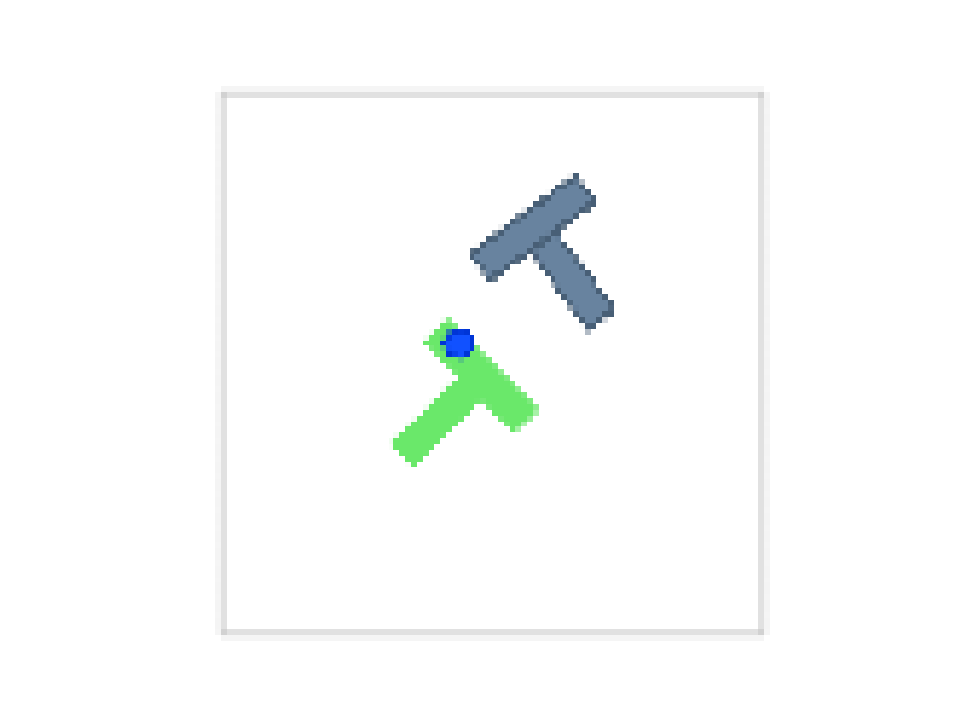
\includegraphics[width=\linewidth]{figures/illustration.pdf}
        \caption{No perturbation}
        \label{fig:visual_perturbations_examples_clean}
    \end{subfigure}
    \begin{subfigure}[b]{0.3\linewidth}
        \centering
        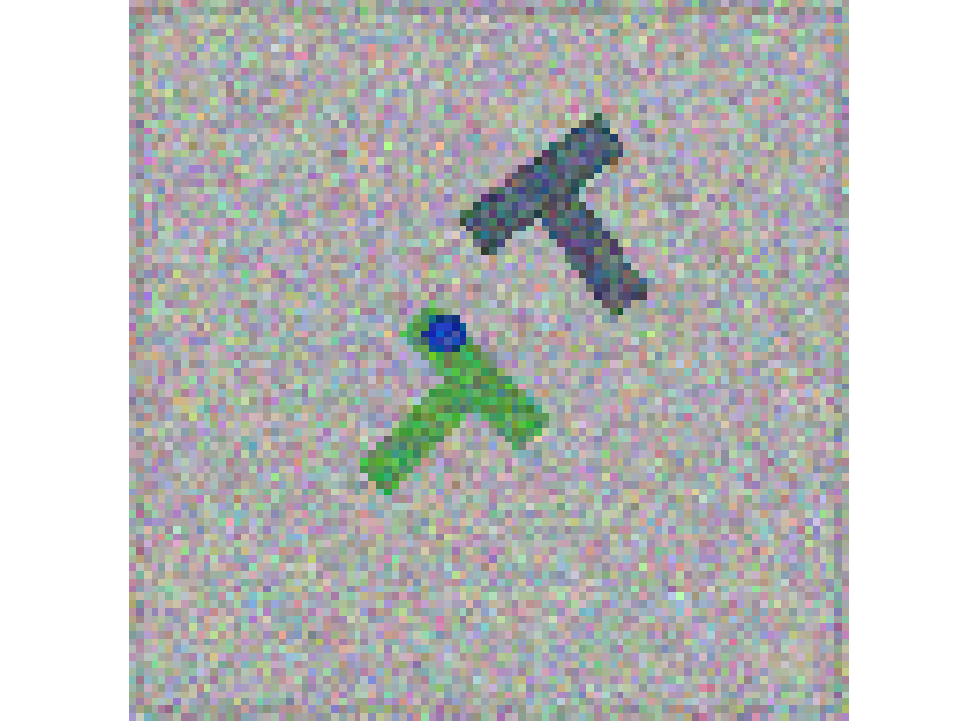
\includegraphics[width=\linewidth]{figures/illustration_noise.pdf}
        \caption{Gaussian noise}
        \label{fig:visual_perturbations_examples_noise}
    \end{subfigure}
    \begin{subfigure}[b]{0.3\linewidth}
        \centering
        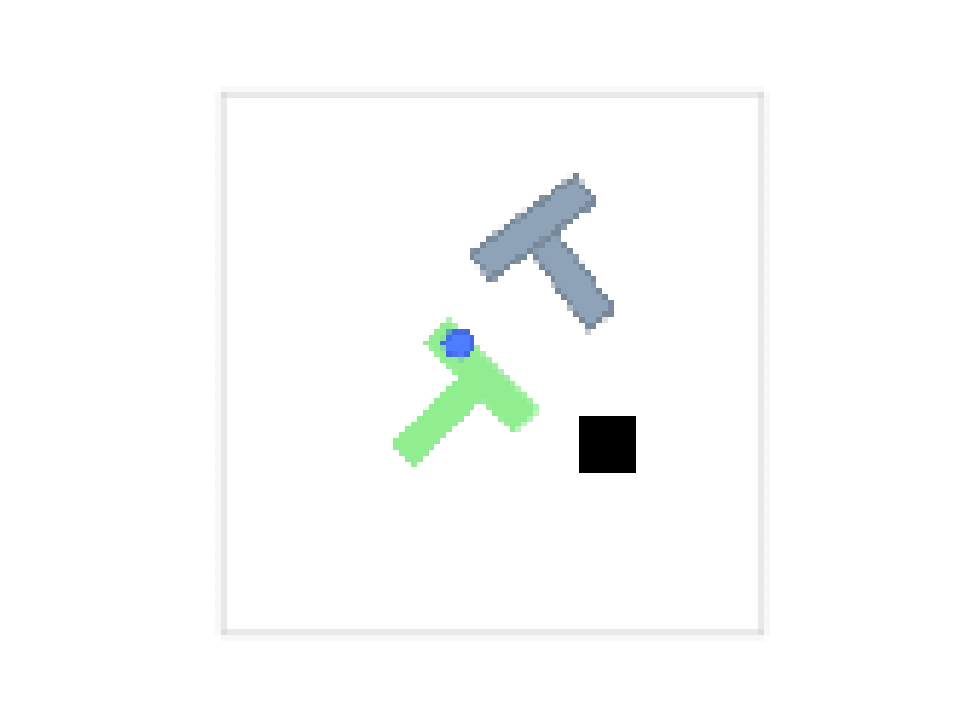
\includegraphics[width=\linewidth]{figures/illustration_patch.pdf}
        \caption{Black patch}
        \label{fig:visual_perturbations_examples_patch}
    \end{subfigure}
    \caption{Example input images for the three considered visual conditions.}
    \label{fig:visual_perturbations_examples}
\end{figure}

By comparing policy performance across these conditions, we aim to draw meaningful conclusions about
the LeRobot provided action diffusion model's visual robustness and more generally, the model's ability to
generalize to unseen scenarios.
% All experiments use consistent evaluation metrics, including task success rate and final object displacement error, to facilitate direct comparisons. The subsequent sections detail the evaluation results and provide insights into the factors influencing the model's robustness.